\documentclass{article}
\usepackage{enumitem}
\usepackage[T1]{fontenc}
\usepackage[utf8]{inputenc}
\usepackage[portuguese]{babel}
\usepackage[vmargin=3cm]{geometry}
\usepackage{tikzpagenodes}
\usepackage{lipsum}
\usepackage{xcolor}
\usepackage{cancel}
\usepackage{amsmath}
\usepackage{amssymb}
\usepackage{background}
\usepackage{titlesec}
\usepackage[nodisplayskipstretch]{setspace}
\usepackage{hyphenat}
\usepackage[normalem]{ulem}
\usepackage{minted}
\usepackage{subcaption}
\hyphenation{mate-mática recu-perar}

\titlespacing{\section}{0pc}{-0.25em}{0pc}
\titlespacing{\subsection}{0pc}{0em}{0pc}
\titlespacing{\subsubsection}{0pc}{0.33em}{0pc}
\titlespacing{\paragraph}{0em}{0.125em}{0.5em}
\setlength{\parindent}{2em}
\setlength{\parskip}{1em}
\linespread{1}

\renewcommand{\baselinestretch}{1.0}

\renewcommand\bf[1]{\textbf{#1}}
\renewcommand\it[1]{\textit{#1}}

\newcommand\ov[1]{\overline{#1}}
\newcommand{\vect}[1]{\mathbf{#1}}
\newcommand{\vn}{\varnothing}
\newcommand\stk[2][black]{\setbox0=\hbox{$#2$}%
\rlap{\raisebox{.45\ht0}{\textcolor{#1}{\rule{\wd0}{1pt}}}}#2}

\makeatletter
\global\let\tikz@ensure@dollar@catcode=\relax
\makeatother

\makeatletter
\def\mcolor#1#{\@mcolor{#1}}
\def\@mcolor#1#2#3{%
  \protect\leavevmode
  \begingroup
    \color#1{#2}#3%
  \endgroup
}
\makeatother
\definecolor{notepadrule}{RGB}{217,244,244}

\backgroundsetup{
contents={%
  \begin{tikzpicture}
    \foreach \fila in {0,...,52}
    {
      \draw [line width=1pt,color=notepadrule]
      (current page.west|-0,-\fila*12pt) -- ++(\paperwidth,0);
    }
    \draw[overlay,red!70!black,line width=1pt]
      ([xshift=-1pt]current page text area.west|-current page.north) --
      ([xshift=-1pt]current page text area.west|-current page.south);
  \end{tikzpicture}%
},
scale=1,
angle=0,
opacity=1
}

\begin{document}

\setlength{\abovedisplayskip}{12pt}
\setlength{\belowdisplayskip}{12pt}
\setlength{\abovedisplayshortskip}{0pt}
\setlength{\belowdisplayshortskip}{0pt}
% \setlength{\baselineskip}{12pt}
\setlength{\jot}{0pt}

\section{Resolução \it{Mounty Hall}}
Vamos supor um espaço amostral para cada estratégia e nomear as portas como $C, E_1$ e $E_2$.
\\
\bf{Não} realizar a troca temos o espaço amostral $S_1 = \{(C,E_1,C), (E_1,E_2,E_1), (E_2,E_1,E_2),
(C,E_2,C)\}$.
\\
Para a troca temos o espaço amostral $S_2 = \{(C,E_1,E_2), (C,E_2,E_1), (E_2,E_1,C),
(E_1,E_2,C)\}$.

Queremos comparar $P_1(\{(C,E_1,C),(C,E_2,C)\})$ e $P_2(\{(E_1,E_2,C), (E_2,E_1,C)\})$

Sabemos que:
\begin{align*}
    P_1(\{(C,E_1,C),(C,E_2,C)\}) = 1/3 \\
    P_1(\{E_1,E_2,E_1\}) = 1/3 \\
    P_1(\{E_2,E_1,E_2\}) = 1/3 \\
    P_2(\{(C,E_1,E_2), (C,E_2,E_1),\}) = 1/3 \\
    P_2(\{(E_1,E_2,C)\}) = 1/3 \\
    P_2(\{(E_2,E_1,C)\}) = 1/3 \\
\end{align*}
Finalmente a melhor escolha é realizar a troca para maximizar as chances de ganhar.

$P_1(\{(C,E_1,C),(C,E_2,C)\}) = 1/3$

$P_2(\{(E_1,E_2,C), (E_2,E_1,C)\}) = 2/3$

\section{Avaliação Empírica da Gaussiana}
Uma função para receber um vetor de realizações e obter a PDF.
\begin{minted}[breaklines, linenos]{matlab}
clear all; close all; clc;
N = 1e6;
nbins = 1000;
x = randn(N, 1);

% Empirical Method
[epdf, bins_centers] = pdf_empirical_evaluation(x, nbins);

% Theoretical Method
m = 0;
v = 1;
tpdf = 1/sqrt(2*pi*v) * exp(-0.5*(bins_centers-m).^2/v);

% Plots
plot(bins_centers, epdf);
hold on; plot(bins_centers, tpdf, 'r--');
legend('Empirical PDF', 'Theoretical PDF');

% Chi-Square Random Variable
y = x.^2;
figure;
[epdfy, bins_centersy] = pdf_empirical_evaluation(y, nbins);
plot(bins_centersy, epdfy);
grid on;
title('Chi-Square Random Variable');

% Mean and Variance
mu_x = sum(x)/length(x);
mu_y = sum(y)/length(y);
disp(['Sample mean of X: ' num2str(mu_x)]);
disp(['Sample variance of X:' num2str( sum((x-mu_x).^2) / (length(x)-1))]); % len-1 -> non-biased estimator
disp(['Sample mean of x: ' num2str(mu_y)]);
disp(['Sample variance of y:' num2str( sum((y-mu_y).^2) / (length(y)-1))]); % len-1 -> non-biased estimator
% >> test_pdf_empirical_evaluation
% Sample mean of X: -0.00085288
% Sample variance of X:0.99913
% Sample mean of x: 0.99913
% Sample variance of y:2.0004

function [epdf, bins_centers] = pdf_empirical_evaluation(x, nbins)
    if ~exist('nbins', 'var') || isempty(nbins)
        nbins = 1000;
    end
    [h, bins_centers] = hist(x, nbins);
    bin_width = (bins_centers(2:end) - bins_centers(1:end-1));
    bin_width = mean(bin_width);
    epdf = (h/length(x))/bin_width;
end

\end{minted}

\begin{figure}[H]
    \centering
    \begin{subfigure}[t]{.5\textwidth}
        \centering
        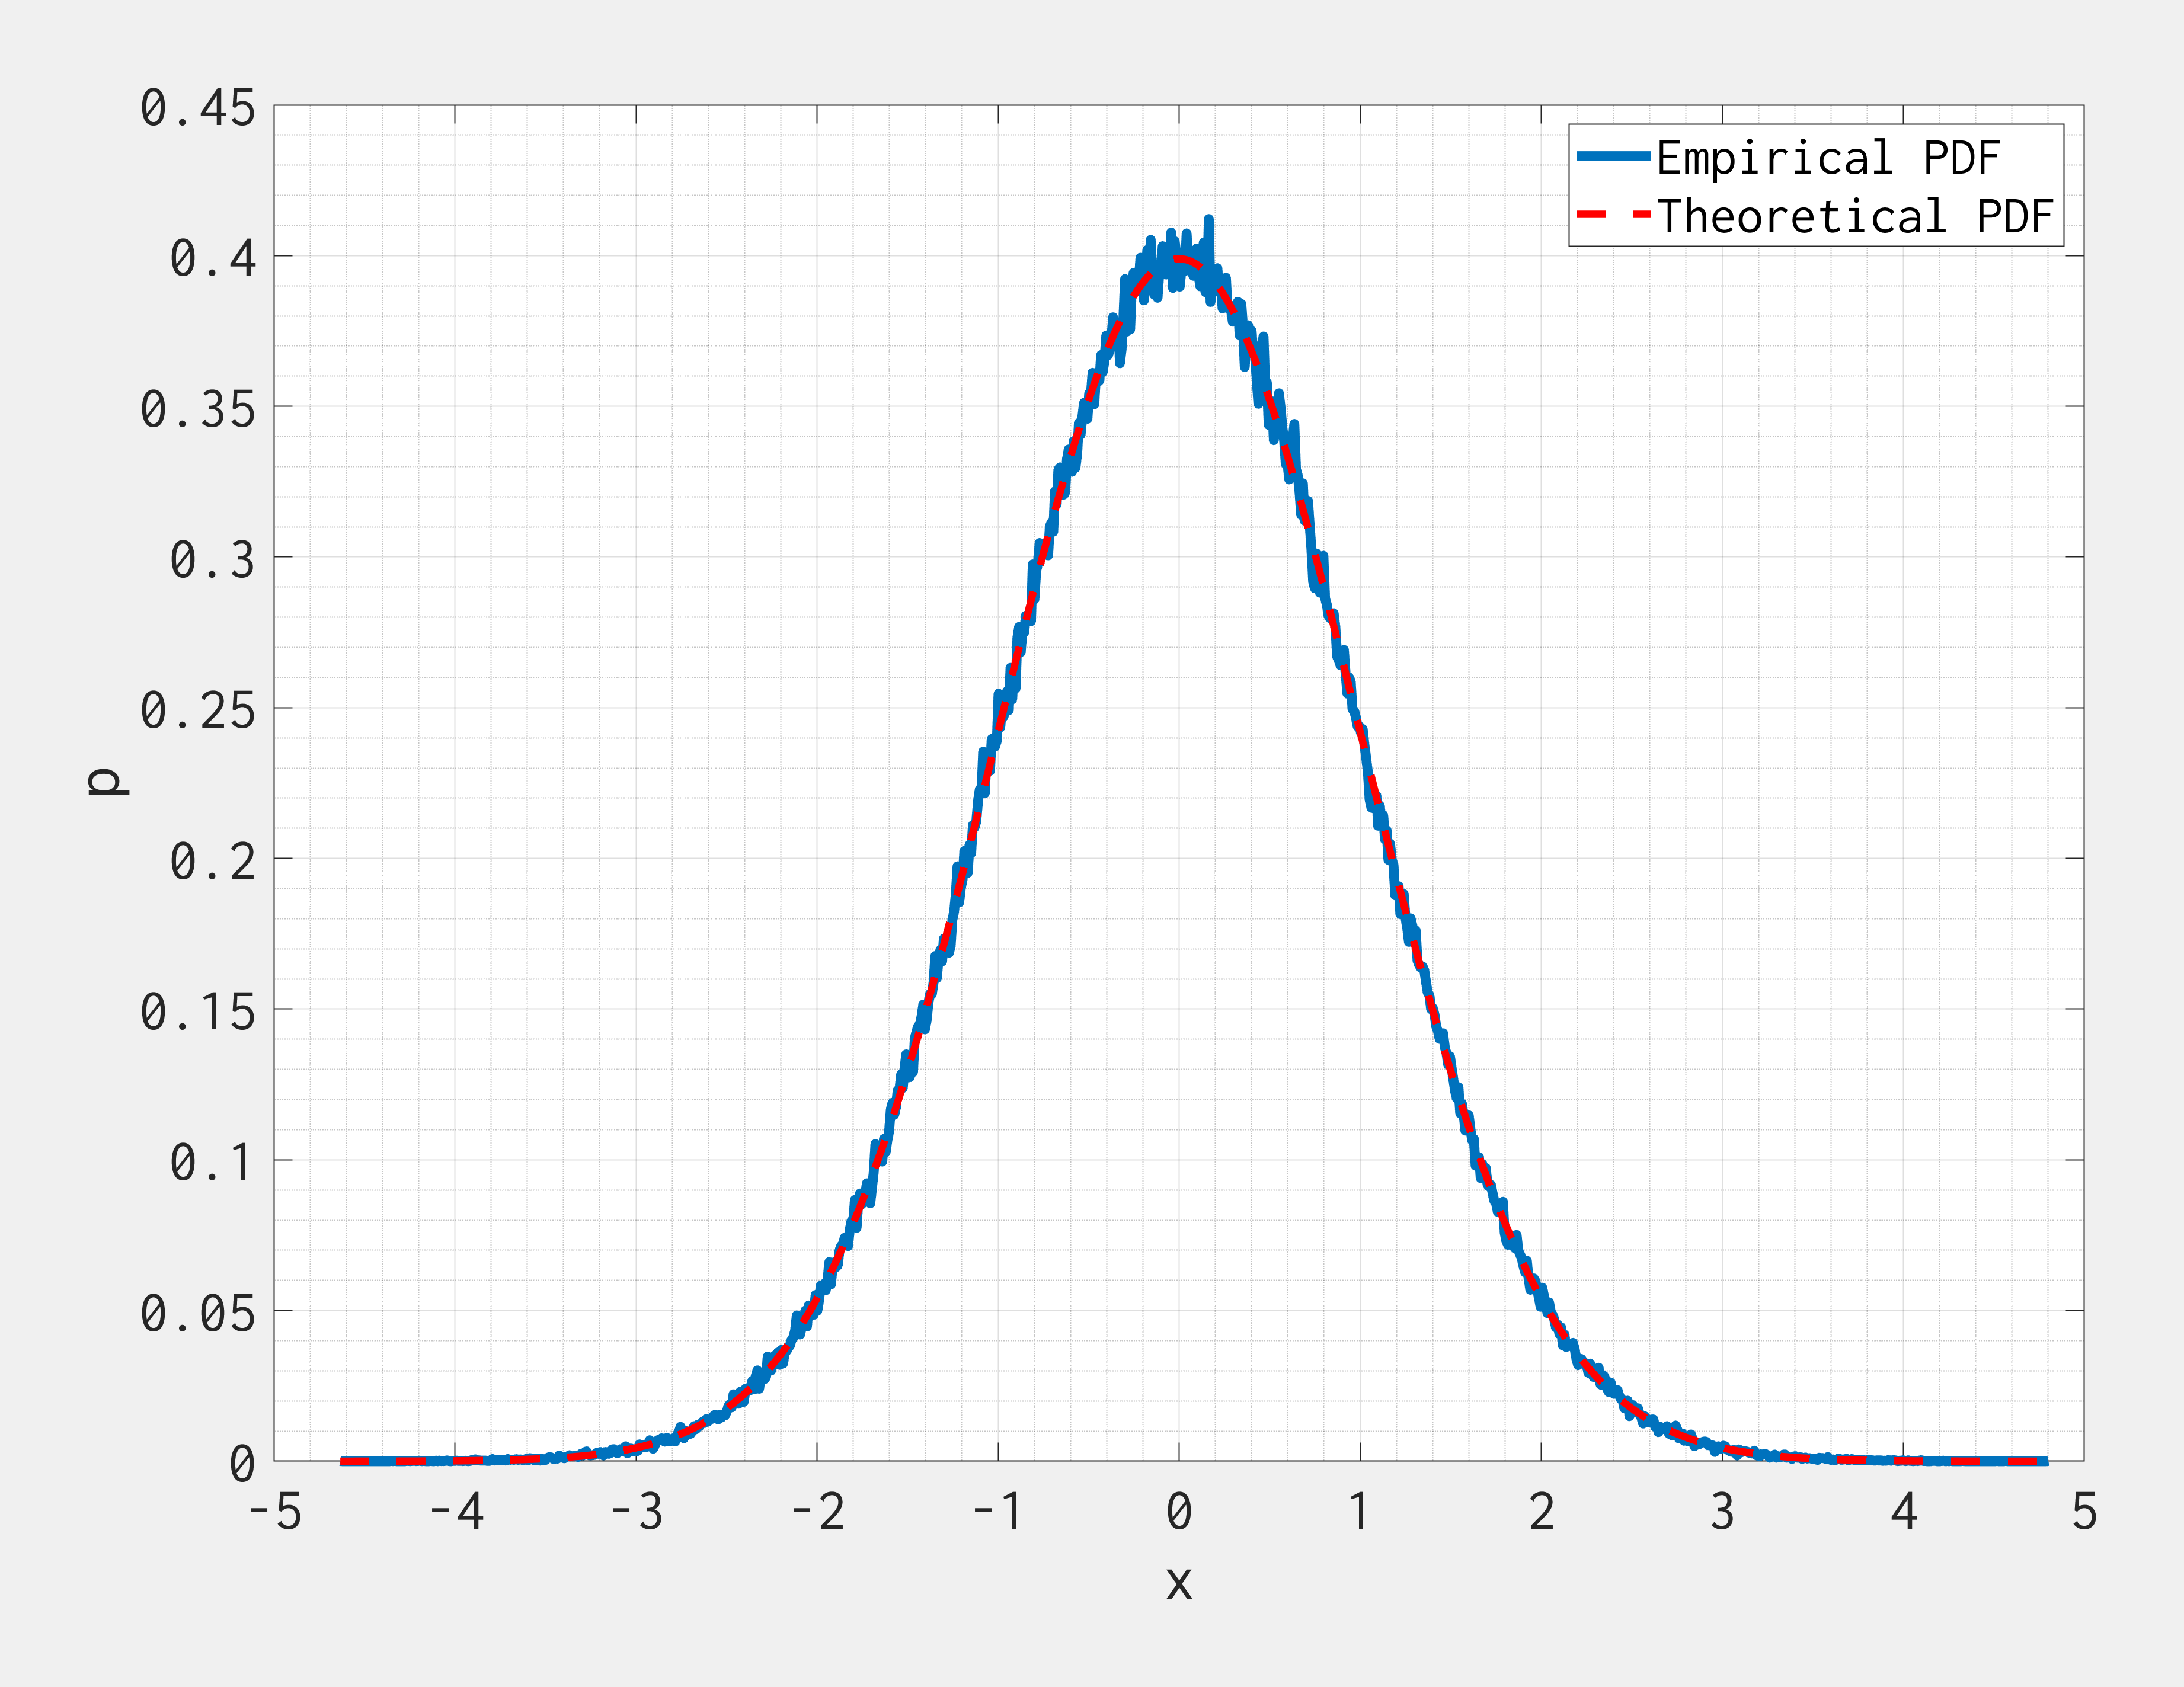
\includegraphics[scale=0.22]{figures/Gaussian-PDF.png}
        \caption{PDF Empírica e Teórica de uma Variável Aleatória Gaussiana Padrão}
    \end{subfigure}%
    \begin{subfigure}[t]{.5\textwidth}
        \centering
        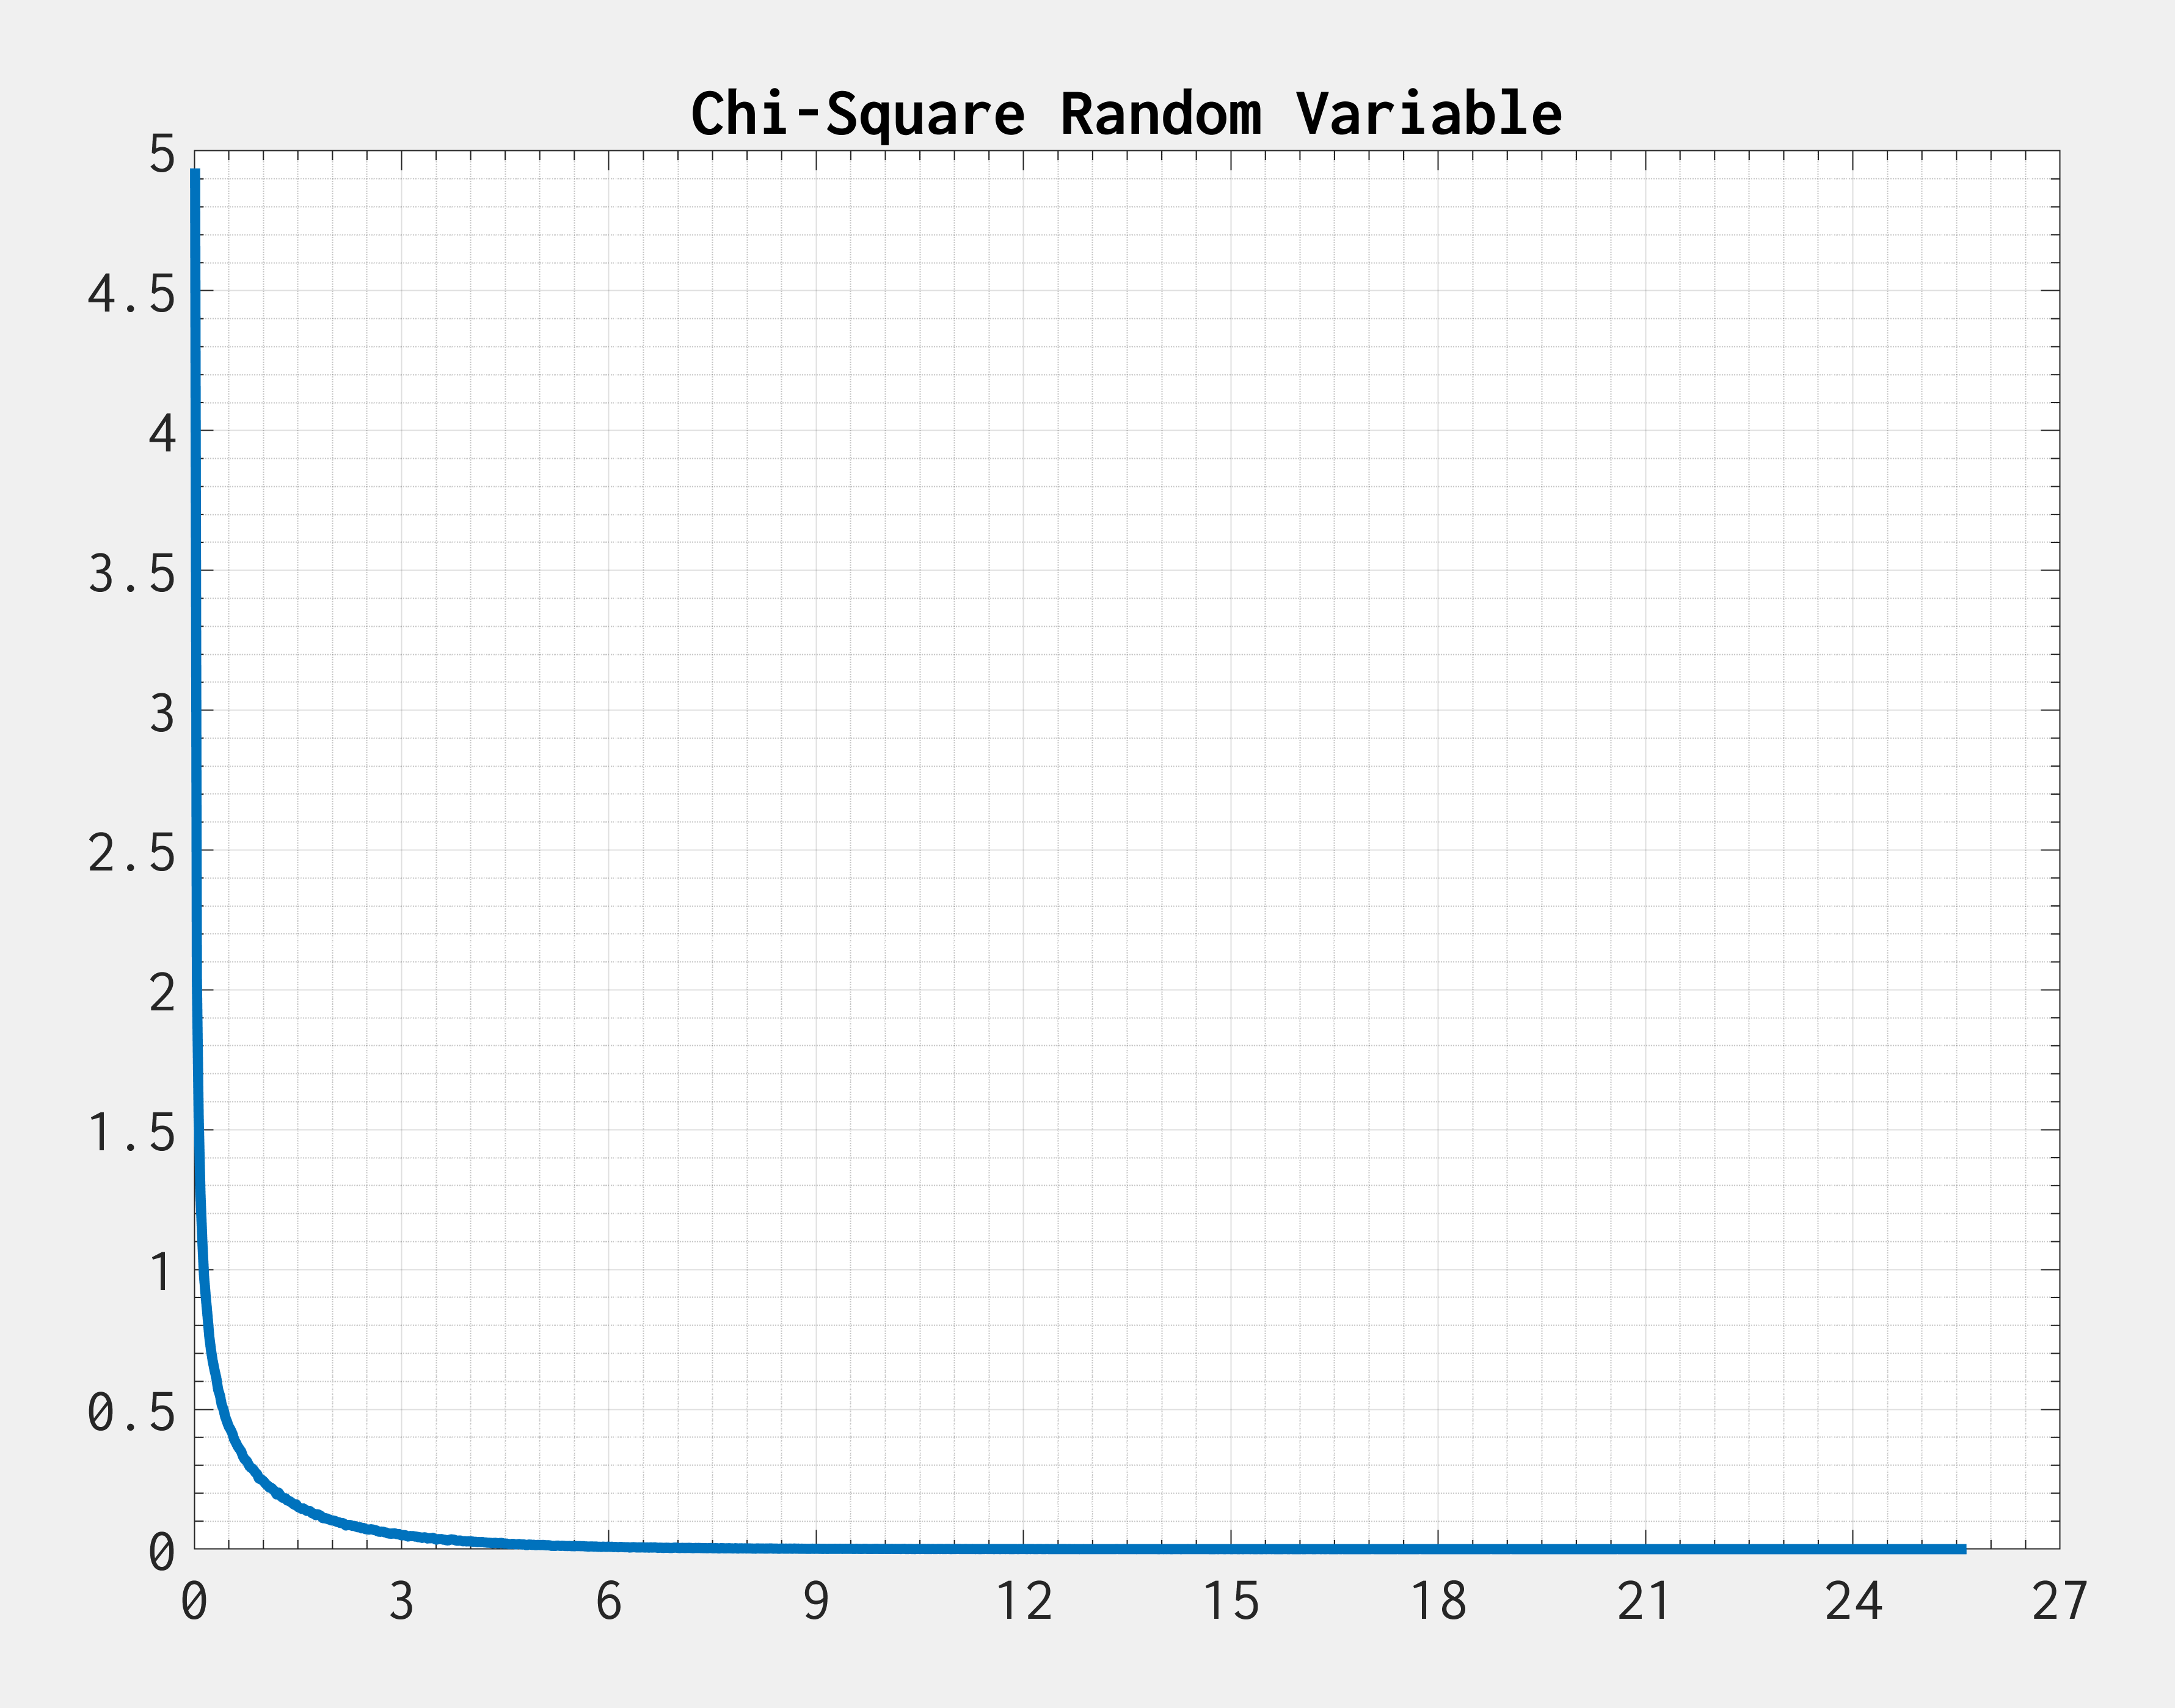
\includegraphics[scale=0.22]{figures/Chi-Square-PDF.png}
        \caption{PDF Empírica de uma Variável Aleatória Chi-Quadrado}
    \end{subfigure}
\end{figure}

\end{document}
